%File: main.tex -- AAAI-2027 (AuthorKit27). The attention-sink / windowed-finetuning paper.
\documentclass[letterpaper]{article} % DO NOT CHANGE THIS
\usepackage[submission]{aaai2027}  % DO NOT CHANGE THIS
\usepackage[hyphens]{url}  % DO NOT CHANGE THIS
\usepackage{graphicx} % DO NOT CHANGE THIS
\urlstyle{rm} % DO NOT CHANGE THIS
\def\UrlFont{\rm}  % DO NOT CHANGE THIS
\usepackage{natbib}  % DO NOT CHANGE THIS AND DO NOT ADD ANY OPTIONS TO IT
\usepackage{caption} % DO NOT CHANGE THIS AND DO NOT ADD ANY OPTIONS TO IT
\frenchspacing  % DO NOT CHANGE THIS
\usepackage{amsmath}
\usepackage{amssymb}
\usepackage{amsfonts}
\usepackage{booktabs}
\usepackage{multirow}
\usepackage{xcolor}
\pdfinfo{
/TemplateVersion (2027.1)
}
\setcounter{secnumdepth}{2}

\title{Context Is the New Weight: Trading the Attention Sink for a Constant Working Memory via Windowed Finetuning}
\author{Zizhao Hu}
\affiliations{
    Department of Computer Science, University of Southern California\\
    zizhaohu@usc.edu
}

\begin{document}
\maketitle

\begin{abstract}
Causal language models develop an \emph{attention sink}: heads route a large fraction of their attention onto the first one or two tokens, regardless of content. We argue this sink is not an accident but a direct consequence of the triangular causal mask --- early positions are visible to every later query, so they accumulate attention --- and that it is precisely what makes a pretrained model fragile to a bounded context: naively restricting attention to a sliding window deletes position~0 and the model collapses. We instead finetune the attention itself under a sliding-window mask, so the model operates with a \emph{constant working memory} of the $W$ most-recent tokens and must offload everything older into its weights --- \emph{context becomes weight}. We study three variants: a plain \textbf{windowed} model, a \textbf{startup} model with a trainable cold-start prompt, and a \textbf{persistent-prompt} model whose prompts are always attendable (trainable attention sinks). On Qwen2.5-0.5B, windowed finetuning recovers near-full-context language-modelling quality at a 256-token window and drives the position-1 sink from $57\%$ of heads to $0\%$; the sink relocates onto the startup prompt. On the hybrid Qwen3.5-9B (only $1/4$ of layers are softmax attention), finetuning just those $8$ layers under a window matches the model's full-context perplexity at a $256$-token window and \emph{beats StreamingLLM without keeping any sink tokens}. A train-window $\times$ inference-window study yields a simple deployment rule --- \emph{train small, deploy anywhere} --- and the persistent-prompt variant turns the sink into $64$ trainable always-on registers that absorb a controllable $19\%$ of attention.
\end{abstract}

\section{Introduction}
Transformer language models are trained with a causal (triangular) attention mask: a query at position $t$ may attend only to keys at positions $\le t$. A robust empirical phenomenon emerges under this mask --- the \emph{attention sink} \citep{xiao2024streamingllm}: across heads and layers, a disproportionate share of attention mass lands on the very first token(s) of the sequence, even when those tokens carry no relevant information. The sink is now understood as a ``no-op'' that heads use to dump attention they do not need, and exploiting it (keeping a few initial tokens) is what lets streaming inference work at all \citep{xiao2024streamingllm,han2024lminfinite}.

We take the sink seriously as a \emph{cause}, not just a curiosity. Two observations motivate this paper. First, the sink is an artifact of the mask geometry: under a triangular mask the first token is in the receptive field of \emph{every} later query, so it is structurally positioned to accumulate attention; the data, by contrast, dilute the first token's importance as context grows. Second, the sink is exactly what breaks a model when we try to bound its memory. If we want a \emph{constant working memory} --- attention restricted to the $W$ most-recent tokens, so that compute and KV-cache are $O(W)$ rather than $O(t)$ --- then a plain sliding window deletes position~0, removes the sink, and the pretrained model collapses.

The standard response is to keep the sink at inference time (StreamingLLM: retain a few initial ``sink'' tokens plus the recent window) \citep{xiao2024streamingllm}. We ask a different question: \emph{can we finetune the sink away?} If the model is trained under the sliding-window mask, every token must learn to predict from a bounded window, and any long-range information it still needs has to be written into the \emph{weights} rather than read from far-away keys. This is the sense in which ``context is the new weight'': adaptation that an in-context model performs by attending to distant tokens is, after windowed finetuning, performed by the parameters.

We make the following contributions:
\begin{itemize}
\item We \textbf{disentangle two types of attention sink} that prior work conflates --- a \emph{positional} sink on the first token and a \emph{no-op} sink on low-information tokens (commas, periods) --- and show they are caused by two \emph{different mechanisms}: the positional sink by the triangular mask's exposure imbalance, the no-op sink by content-driven bounded-memory token usage (Sec.~\ref{sec:sink}--\ref{sec:hyp}). We show by finetuning that the positional sink is \emph{learned and removable} --- a windowed mask drives it to zero --- while the no-op sink remains and is leaned on more.
\item We introduce three windowed-finetuning variants --- \textbf{windowed}, \textbf{startup} (a trainable cold-start prompt), and \textbf{persistent-prompt} (always-on trainable registers) --- that give a model a constant working memory (Sec.~\ref{sec:method}).
\item On Qwen2.5-0.5B and the hybrid Qwen3.5-9B we show that windowed finetuning recovers near-full-context perplexity at a $256$-token window, beats StreamingLLM \emph{without} sink tokens, and obeys a clean ``train small, deploy anywhere'' rule (Sec.~\ref{sec:exp}).
\end{itemize}

\section{Two Types of Attention Sink}
\label{sec:sink}
We distinguish two distinct phenomena that are both commonly called ``attention sinks.'' They differ in \emph{where} the attention lands and in \emph{what} drives it, and the rest of the paper turns on telling them apart.

\paragraph{Type~1 --- the positional sink.} A large, almost content-independent share of every query's attention falls on the first one or two tokens of the sequence, regardless of their content. Figure~\ref{fig:base_sink} shows this for a base model: the leftmost column of the attention map is a bright vertical stripe, and token~1 absorbs on average $0.42$ of the attention mass --- an order of magnitude more than any later key --- across a majority of heads. This is the sink exploited by StreamingLLM \citep{xiao2024streamingllm}: it is tied to absolute \emph{position}, not to meaning.

\begin{figure}[t]
\centering
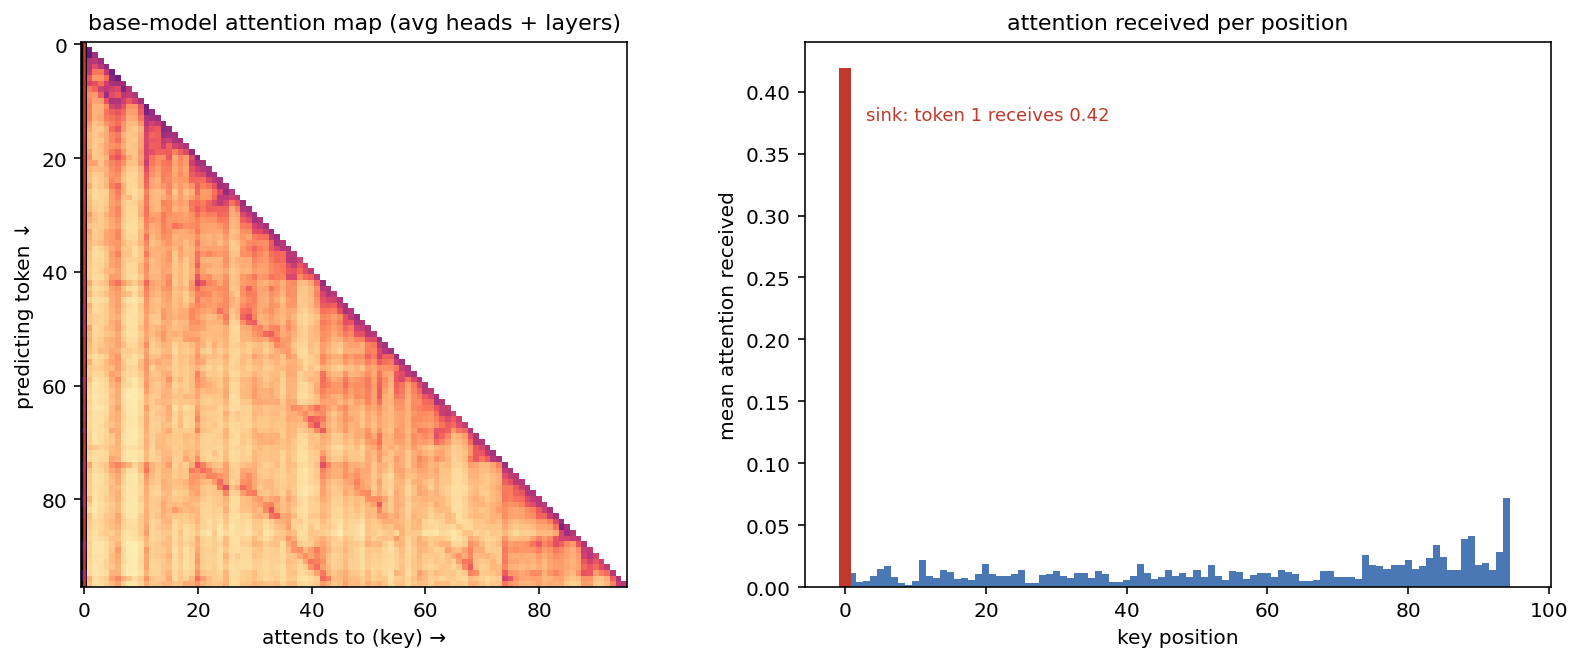
\includegraphics[width=\linewidth]{figures/base_sink.png}
\caption{Type~1 (positional) sink in a base causal LM. \emph{Left:} attention map (averaged over heads and layers); the first column is a bright vertical stripe. \emph{Right:} mean attention received per key position --- token~1 absorbs $0.42$, every other token $<0.05$.}
\label{fig:base_sink}
\end{figure}

\paragraph{Type~2 --- the no-op (low-information) sink.} A second sink falls not on the first position but on semantically near-empty tokens \emph{within} the sequence --- punctuation such as commas and periods, delimiters, and other filler. These tokens carry little predictive information of their own; a head with nothing to retrieve at a given step dumps its attention onto the nearest such token, using it as a local ``no-op'' or scratch register. Unlike Type~1, the no-op sink is distributed throughout the text and keyed to token \emph{identity} rather than to absolute position.

\paragraph{Prior work does not disentangle the two.} Existing accounts of the attention sink have observed \emph{both} behaviours --- the large share of attention parked on the initial token(s) \citep{xiao2024streamingllm,han2024lminfinite} and the attention absorbed by low-information delimiter tokens such as commas and periods --- and have gone as far as describing both as ``no-op'' functionalities a head uses to discard attention. They stop there: the two are folded into a single ``attention sink,'' neither separated from one another nor traced to distinct causes. Our central claim is that they are in fact \emph{disentanglable} and arise from \emph{two different mechanisms}. Type~1 is an artifact of the triangular mask's positional exposure imbalance (H1): it is a property of the \emph{architecture}, and it disappears when the mask changes. Type~2 is a content-driven no-op keyed to token \emph{identity} (H2): it is a property of the \emph{data and the model's use of it}, and it persists --- indeed is leaned on \emph{more} --- once Type~1 is removed (H3). Separating the two is what lets us remove the harmful, mask-induced sink while keeping (and exploiting) the useful one. We state these mechanisms as testable hypotheses next.

\section{Hypotheses}
\label{sec:hyp}

\paragraph{H1: the positional sink is an artifact of the triangular mask.} Under a length-$C$ causal mask a key at position $p$ is attended by the $C-p$ queries after it, so the first token sits in the receptive field of \emph{every} later query --- the maximal possible exposure --- while its data-side importance is only $\propto 1/C$ and \emph{shrinks} with context. We hypothesize that this exposure imbalance biases training to recruit the earliest positions as a stable, content-free information store, producing the Type~1 sink (a degenerate no-op anchor). Consistent with this, the measured sink \emph{grows} with context (Fig.~\ref{fig:sink_cmp}): the model sinks \emph{against} the data-side dilution rather than reflecting it, the signature of an active mechanism rather than a property of the data.

\begin{figure}[t]
\centering

\includegraphics[width=\linewidth]{figures/sink_comparison.png}
\caption{The measured Type~1 sink grows with context length, the opposite of the data-side first-token importance ($\propto 1/C$) --- the model sinks \emph{against} the data, an artifact of the mask (H1).}
\label{fig:sink_cmp}
\end{figure}

\paragraph{H2: the no-op sink lands on non-meaningful tokens.} We hypothesize that Type~2 is the model's mechanism for ``attend to nothing in particular'': heads route attention to low-information tokens --- commas, periods, delimiters --- as content-based no-op sinks, a behaviour driven by token identity and independent of absolute position.

\paragraph{H3: removing Type~1 makes the model reuse the no-op sinks for storage.} If the Type~1 positional bias is removed --- e.g.\ by a windowed objective that masks position~$0$ out of every deep query's receptive field --- the storage/no-op function is not lost. We hypothesize the model instead repurposes the Type~2 low-information tokens to additionally carry the role the position-$0$ sink used to play, storing and relaying information on them rather than on a single distant anchor.

\paragraph{H4: no-op sinks are better information relays for streaming.} Because Type~2 tokens are distributed through the text --- each one sitting at the end of a span of already-accumulated context --- information parked on them has a better context-accumulation property than a single far-away position-$0$ anchor. In a streaming / bounded-window deployment a recent low-information token is always inside the window and has already integrated its local context, making it a better information-relay point than a position-$0$ sink that the window has scrolled past. The constant-working-memory regime should therefore not merely tolerate the loss of the Type~1 sink but \emph{benefit} from leaning on Type~2 relays instead.

\paragraph{Why this matters for bounded memory.} A constant working memory restricts attention to a window of the $W$ most-recent tokens. For a query deep in the sequence this window no longer contains position~$0$, so the Type~1 sink is gone; a pretrained model that relies on it produces degenerate distributions and its perplexity explodes. StreamingLLM \citep{xiao2024streamingllm} patches this at inference by always retaining a few initial tokens. We instead remove the dependency by training (Section~\ref{sec:method}), and ask whether the model falls back on the Type~2 no-op sinks (H3) and whether doing so improves streaming behaviour (H4).

\section{Method: Windowed Attention Finetuning}
\label{sec:method}
Let the causal mask be $M_{\text{causal}}(t,k)=1$ iff $k\le t$. We replace it during finetuning with a sliding-window mask
\[
M_{\text{win}}(t,k)=\mathbb{1}\!\left[\,t-W < k \le t\,\right],
\]
so each token attends only to the $W$ most-recent positions. We finetune (continued pretraining on generic text, language-modelling loss only --- no task supervision) so that the comparison isolates the effect of the \emph{mask}, not of any downstream data. We study three schemes (Fig.~\ref{fig:windowed}):

\begin{description}
\item[Windowed.] The plain sliding window above. The window's cold start (the first $W{-}1$ positions, whose window is not yet full) is filled with real preceding tokens during training.
\item[Startup.] We prepend $P$ trainable soft prompts that fill the window's cold start in place of real history, then window over the prompt$+$content sequence. The prompt slides out of the window for deep tokens, so it functions purely as a learned cold-start anchor --- a trainable replacement for the sink token. This grants \emph{availability}: the model can be deployed from token~1 without needing $W$ real tokens of history.
\item[Persistent prompt.] We prepend $P$ trainable prompts that are \emph{always} attendable by every content token (a persistent learned prefix), while the content is windowed to $W$. Each token then sees $W$ recent tokens \emph{plus} $P$ constant learned registers (effective memory $W{+}P$, of which $P$ is fixed). The prompts become trainable, always-on attention sinks.
\end{description}

\begin{figure}[t]
\centering

\includegraphics[width=\linewidth]{figures/windowed_attention.png}
\caption{Windowed attention finetuning. The triangular mask (left) is replaced by a sliding window (a band of width $W$), giving each token a constant working memory of the recent $W$ tokens; older context must be carried by the weights.}
\label{fig:windowed}
\end{figure}

\section{Experiments}
\label{sec:exp}
We evaluate on Qwen2.5-0.5B (a pure-softmax-attention model, our proof of concept) and Qwen3.5-9B (the target model). Finetuning is continued pretraining on WikiText-103 \citep{merity2017wikitext}; evaluation is held-out perplexity scored within a working-memory window, plus downstream long-context QA on LongBench \citep{bai2024longbench}. Unless noted, the window for the headline runs is $W{=}256$.

\subsection{Windowed Finetuning Recovers Full-Context Quality}
On Qwen2.5-0.5B, scoring held-out perplexity as a function of the deployed window shows the expected collapse for a base model windowed at inference, and a near-flat curve for the windowed-finetuned model (Fig.~\ref{fig:ppl}): a model trained for a $256$-token window matches the base model's full-context quality while attending to $8{\times}$ fewer tokens (Table~\ref{tab:ppl05b}). Continued pretraining under \emph{full} attention does not help --- it amplifies sink reliance --- whereas the windowed objective removes it.

\begin{figure}[t]
\centering
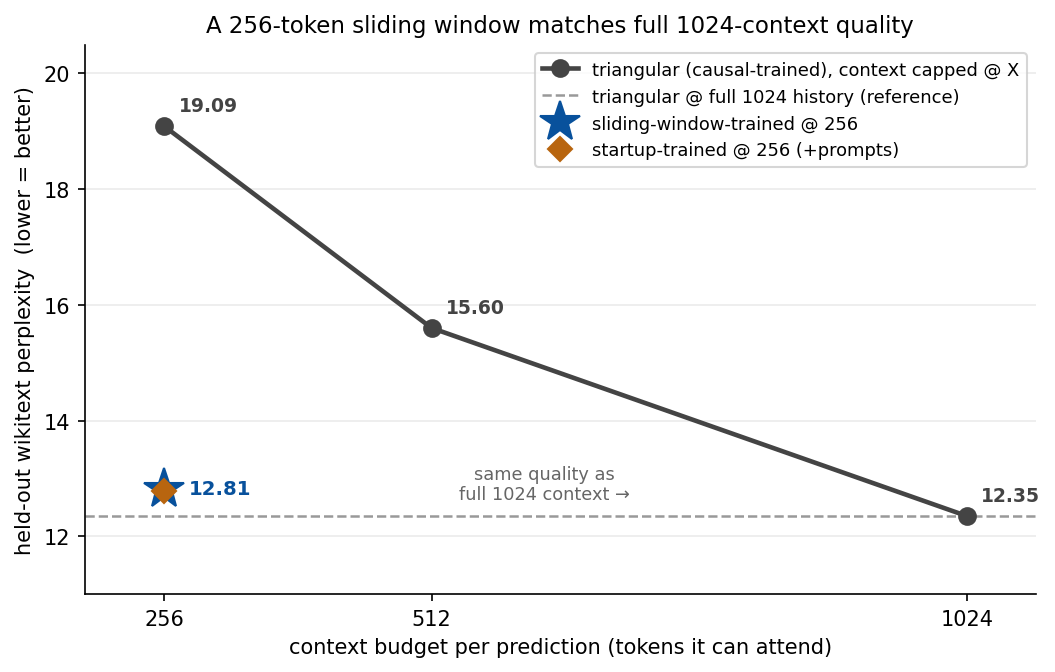
\includegraphics[width=\linewidth]{figures/ppl_curve.png}
\caption{Held-out perplexity vs.\ deployed working-memory window (Qwen2.5-0.5B). The base model collapses as the window shrinks; the windowed-finetuned model is nearly flat and matches full-context quality at a small window.}
\label{fig:ppl}
\end{figure}

\begin{table}[t]
\centering
\small
\begin{tabular}{lcc}
\toprule
model (Qwen2.5-0.5B) & context budget & held-out ppl \\
\midrule
triangular (causal-trained) & 256 & 19.09 \\
triangular (causal-trained) & 512 & 15.60 \\
triangular (causal-trained) & 1024 (full) & \textbf{12.35} \\
sliding-window-trained & 256 & \textbf{12.81} \\
startup-trained & 256\,($+$\,prompts) & 12.78 \\
\bottomrule
\end{tabular}
\caption{Held-out wikitext perplexity vs.\ context budget on Qwen2.5-0.5B. The causal-trained model needs the full 1024-token history (12.35) and degrades steeply when windowed (19.09 at 256 --- worse than the untrained base, because windowing masks the first-token sink it leans on); the windowed-finetuned model reaches 12.81 at a 256-token window, matching the causal model's full-context quality on a quarter of the context.}
\label{tab:ppl05b}
\end{table}


\subsection{The Sink Is Learned and Removable}
Measuring the position-1 sink before and after finetuning shows it is a learned behaviour. On Qwen2.5-0.5B, a majority of softmax heads ($\approx 57\%$) sink onto token~1 in the base and full-attention-finetuned models; windowed finetuning drives this to $0\%$ (Table~\ref{tab:sink05b}), and the \textbf{startup} variant relocates the sink onto the trainable prompt rather than the content. On the larger hybrid model the absolute sink is weaker (see below) but the \emph{direction} is identical: full-attention finetuning \emph{builds} the sink, windowed finetuning \emph{shrinks} it (Fig.~\ref{fig:9bsink}).

\begin{figure}[t]
\centering
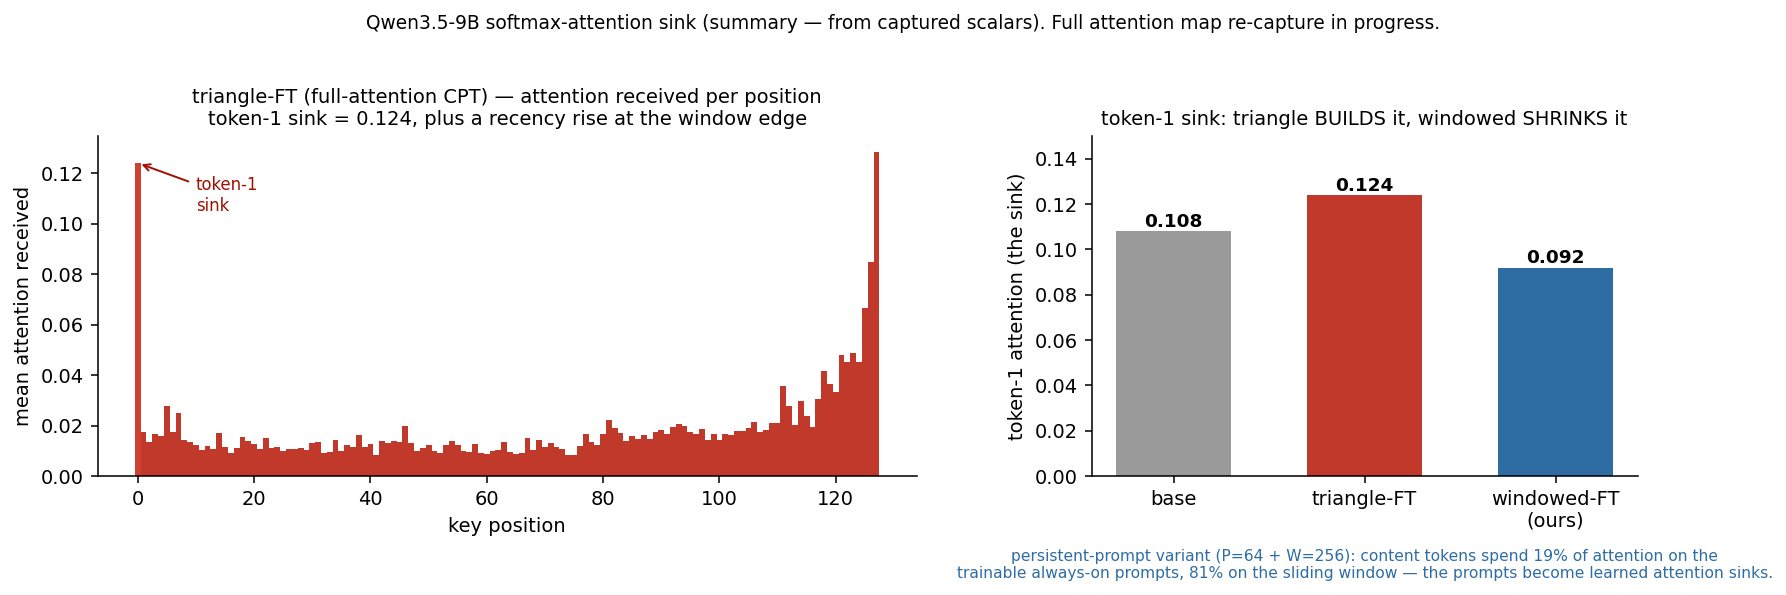
\includegraphics[width=\linewidth]{figures/qwen9b_sink_summary.png}
\caption{Qwen3.5-9B softmax-layer sink. Full-attention (triangle) finetuning builds the token-1 sink to $0.124$; windowed finetuning shrinks it to $0.092$; base is between ($0.108$). The persistent-prompt variant relocates $\sim$$19\%$ of every content token's attention onto trainable always-on registers.}
\label{fig:9bsink}
\end{figure}

\begin{table}[t]
\centering
\small
\begin{tabular}{lcc}
\toprule
 & full attention & sliding-window mask \\
 & (learned tendency) & (as deployed) \\
\midrule
base $+$ history & 57.6\% & 0.0\% \\
sliding-history (trained) & \textbf{5.8\%} & 0.0\% \\
\bottomrule
\end{tabular}
\caption{Position-1 sink on Qwen2.5-0.5B given the \emph{same} real history (63 history $+$ 256 content, $W{=}64$): \% of softmax heads with mean attention $>0.3$ to the history's first token. Sliding-window finetuning cuts the learned sink $\sim$$10\times$ (57.6\%$\to$5.8\%); the window masks it to 0\% at deployment.}
\label{tab:sink05b}
\end{table}


\subsection{Where the Attention Goes: Type-1 to Type-2}
Removing the Type-1 sink does not destroy the attention mass --- it \emph{relocates} it. On Qwen2.5-0.5B we measure, under each scheme's deployment, the fraction of attention received by the first token (Type-1) versus low-information punctuation tokens (Type-2), and the entropy of the per-position attention (Table~\ref{tab:spread}, Fig.~\ref{fig:spread}). Continued full-causal (triangle) training keeps the Type-1 sink ($0.41$); windowed and startup training drain it (to $0.15$ and $0.008$) and the freed mass lands on the distributed Type-2 punctuation tokens ($0.17\!\to\!0.37$), with the broadcasting entropy rising $3.9\!\to\!5.0$. This is exactly H2--H3: with the positional sink suppressed, the model reuses the content-based no-op tokens and spreads attention more broadly. We note a limit (below): this broader spread is a \emph{distributional} property, not long-range retrieval.

\begin{table}[t]
\centering
\small
\setlength{\tabcolsep}{4pt}
\begin{tabular}{lcccc}
\toprule
 & Type-1 & \multicolumn{2}{c}{Type-2 (no-op)} & broadcast \\
\cmidrule(lr){3-4}
scheme & (pos-0) & punct.\ & low-surp.\ & entropy \\
\midrule
base         & 0.368 & 0.146 & 0.148 & 4.51 \\
triangle-CPT & 0.383 & 0.137 & 0.138 & 4.43 \\
sliding-history     & 0.151 & 0.323 & 0.354 & 5.18 \\
uniform-context. & 0.202 & 0.130 & 0.160 & 5.41 \\
trainable startup      & \textbf{0.004} & \textbf{0.396} & \textbf{0.449} & \textbf{5.52} \\
\bottomrule
\end{tabular}
\caption{Where attention goes (Qwen2.5-0.5B; all schemes measured identically at a \emph{genuine} $256$-token window over $512$-token sequences). Fraction of attention received by the position-0 token (Type-1) vs.\ low-information no-op tokens (Type-2), the latter measured two ways, a fixed punctuation list and the bottom-$20\%$ unigram-surprisal tokens, which agree, so the no-op sink is not an artifact of the punctuation proxy. Continued full-causal (triangle) training keeps (slightly intensifies) the Type-1 sink; sliding-history and trainable startup training drain it onto the distributed Type-2 tokens and raise the broadcasting entropy. The \emph{uniform-context} model is an instructive exception: it reduces Type-1 (to $0.20$) and raises the entropy, but the freed mass does \emph{not} land on the Type-2 separators (punct.\ and low-surp.\ stay near base), spreading diffusely instead. The attention--surprisal correlation sharpens in step ($-0.07$ at base $\to$ $-0.16$ at trainable startup): as Type-1 dies, attention concentrates more on low-information tokens.}
\label{tab:spread}
\end{table}


\begin{figure}[t]
\centering
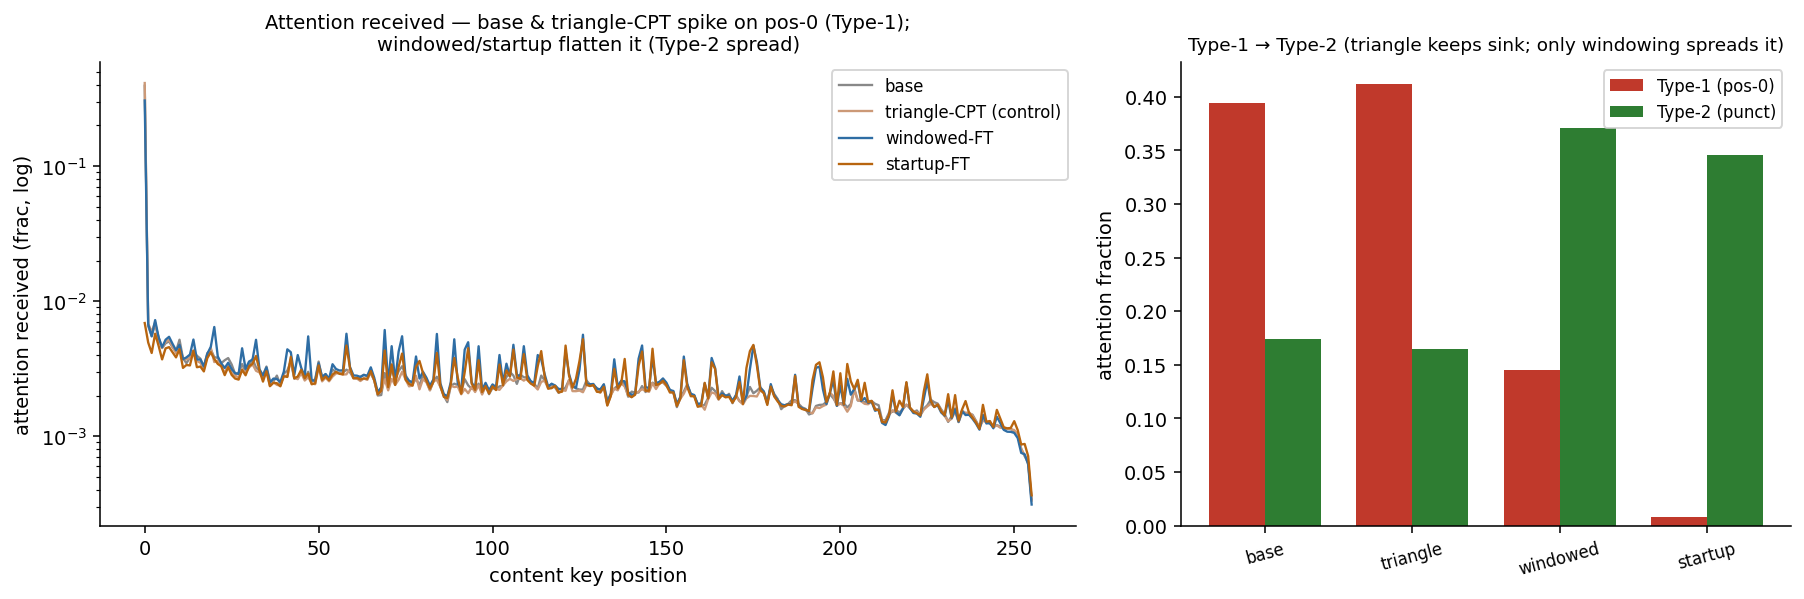
\includegraphics[width=\linewidth]{figures/qwen_sink_spread.png}
\caption{Windowed/startup training drains the Type-1 positional sink (left, log scale: base spikes $\approx0.39$ at position~0; windowed/startup flatten it) and redistributes the mass onto distributed Type-2 punctuation tokens (right), broadcasting entropy rising $3.9\!\to\!5.0$.}
\label{fig:spread}
\end{figure}

\subsection{Scaling to a Hybrid Model}
Qwen3.5-9B is a hybrid: of its $32$ layers, only $8$ (every $4$th) are softmax attention; the rest are linear/Mamba-style attention \citep{gu2024mamba,gu2025gateddeltanet}. The sink, and the windowing question, therefore concern only those $8$ layers --- $3/4$ of the network is already a constant-memory mechanism. We full-finetune just the $8$ softmax blocks (freezing the $24$ linear layers; $8$-bit AdamW with gradient checkpointing on a single $48$\,GB GPU). Even on this model, bounding the softmax window to $256$ tokens collapses the base from a full-context perplexity of $6.5$ to $20.0$; windowed finetuning restores it to $6.3$ --- full-context quality at a $256$-token softmax window --- and, unlike the baselines, gains nothing from StreamingLLM sink tokens because it no longer depends on them (Table~\ref{tab:matrix}).

\begin{table}[t]
\centering
\small
\setlength{\tabcolsep}{4pt}
\begin{tabular}{lccccc}
\toprule
& \multicolumn{5}{c}{perplexity at inference window} \\
\cmidrule(lr){2-6}
model & 128 & 256 & 512 & 1024 & 2048 \\
\midrule
\multicolumn{6}{l}{\emph{untrained baseline}}\\
base 9B            & 59.8 & 28.1 & 13.8 & 7.80 & 7.26 \\
\;+ StreamingLLM   & 9.33 & 8.47 & 7.91 & 7.58 & 7.28 \\
\multicolumn{6}{l}{\emph{continued-pretraining baseline}}\\
triangle-FT        & 33.7 & 18.2 & 8.66 & 6.96 & 6.59 \\
\;+ StreamingLLM   & 7.88 & 7.39 & 7.03 & 6.83 & 6.56 \\
\multicolumn{6}{l}{\emph{ours, windowed (one model per training window)}}\\
windowed-128       & \textbf{7.44} & 7.14 & 6.94 & 6.83 & 6.62 \\
windowed-256       & 7.82 & \textbf{7.19} & 6.93 & 6.79 & 6.57 \\
windowed-512       & 11.5 & 7.82 & \textbf{6.95} & 6.79 & 6.55 \\
windowed-1024      & 24.7 & 12.7 & 7.44 & \textbf{6.83} & 6.54 \\
windowed-2048      & 27.6 & 14.5 & 7.76 & 6.84 & \textbf{6.53} \\
\multicolumn{6}{l}{\emph{ours, startup (windowed + cold-start prompt)}}\\
startup-256        & 7.82 & 7.17 & 6.92 & 6.79 & 6.57 \\
\bottomrule
\end{tabular}
\caption{Qwen3.5-9B held-out perplexity, train-window (rows) $\times$ inference-window (columns); bold is native (train $=$ deploy). Windowed models beat both baselines and their StreamingLLM versions at tight windows, with no sink tokens. Small-window models are robust to any deployment window; wide-window models break when deployed narrower (\emph{train small, deploy anywhere}).}
\label{tab:matrix}
\end{table}


\subsection{Train Small, Deploy Anywhere}
Evaluating every windowed model at every inference window (Table~\ref{tab:matrix}) reveals an asymmetry. A model trained at a \emph{small} window (windowed-128) is nearly flat across \emph{all} deployment windows ($7.44\!\to\!6.62$): having learned to predict from $128$ tokens, it is robust to any budget. A model trained at a \emph{wide} window is fragile when deployed narrower (windowed-1024 rises to $24.7$ at deploy-128), because it learned to lean on context that is no longer present. A model is always fine deployed \emph{wider} than it was trained, and breaks deployed \emph{narrower}: the practical rule is to train at the smallest window one might deploy.

\subsection{A Strict Softmax-vs-Gated Control}
Is the gain from \emph{windowing}, or merely from more finetuning? We answer with a strict control: two $1.3$B models from the flash-linear-attention suite trained on the \emph{same} $100$B tokens with the \emph{same} skeleton, differing only in the token-mixer --- a softmax Transformer and a gated-linear (GLA) model --- evaluated across the full train-window $\times$ deploy-window grid (Table~\ref{tab:strictmatrix}). The softmax base collapses at tight windows ($10.2\!\to\!17.9$ at deploy-$128$); continued \emph{full-causal} pretraining (triangle-CPT) only partly recovers ($14.0$, the control held fixed); windowed finetuning gives near-flat rows --- the same \emph{train small, deploy anywhere} asymmetry as the hybrid model --- so the recovery is from the window, not the extra training. The gated GLA is \emph{window-invariant} ($8.71$ at every budget, having no attention window) and best in every column: native constant-memory attention is the ceiling, and a windowed softmax retrofit is the closest one gets to it without changing the architecture.

\begin{table}[t]
\centering
\small
\setlength{\tabcolsep}{4pt}
\begin{tabular}{lccccc}
\toprule
& \multicolumn{5}{c}{perplexity at inference window} \\
\cmidrule(lr){2-6}
model & 128 & 256 & 512 & 1024 & full \\
\midrule
\multicolumn{6}{l}{\emph{softmax transformer --- untrained / full-mask control}}\\
base               & 17.9 & 14.9 & 12.8 & 11.3 & 10.2 \\
triangle-CPT       & 14.0 & 12.1 & 10.8 & 9.61 & 8.80 \\
\multicolumn{6}{l}{\emph{softmax transformer --- ours, windowed (one model per training window)}}\\
windowed-128       & \textbf{10.6} & 9.70 & 9.30 & 9.10 & 9.06 \\
windowed-256       & 10.8 & \textbf{9.63} & 9.17 & 8.96 & 8.92 \\
windowed-512       & 11.9 & 9.85 & \textbf{9.15} & 8.89 & 8.84 \\
windowed-1024      & 12.7 & 10.5 & 9.36 & \textbf{8.88} & 8.81 \\
\midrule
\multicolumn{6}{l}{\emph{gated (GLA) --- same skeleton \& data, constant memory}}\\
gla                & 8.71 & 8.71 & 8.71 & 8.71 & 8.71 \\
\bottomrule
\end{tabular}
\caption{Strict control on the flash-linear-attention $1.3$B pair (same GPT skeleton, same $100$B training tokens; only the token-mixer differs --- softmax vs.\ gated-linear), held-out perplexity, train-window (rows) $\times$ inference-window (columns); bold marks each windowed model's native window (train $=$ deploy). All rows except \emph{base} are continued-pretrained for the same steps. The softmax base collapses at tight windows; the full-mask (triangle) control only partly recovers; windowed finetuning gives near-flat rows --- \emph{train small, deploy anywhere} --- approaching the gated model. The gated GLA is \emph{window-invariant} ($8.71$ at every budget, having no attention window) and best at every column: native constant-memory attention beats a retrofitted softmax window, which is the best one can do without changing the architecture.}
\label{tab:strictmatrix}
\end{table}


\paragraph{Compute.} The payoff is efficiency. Full softmax attention is $O(L^2)$; the windowed and gated mechanisms are $O(L)$. At a $32$k context the windowed model runs $2.7\times$ faster than full attention (Table~\ref{tab:eff}), with linear rather than quadratic growth.

\begin{table}[t]
\centering
\small
\begin{tabular}{lccc}
\toprule
seq.\ length & full & sliding-history & gated \\
\midrule
$8$k & 313 & 226 & 258 \\
$16$k & 797 & 436 & 499 \\
$32$k & 2363 & \textbf{866} & 989 \\
\bottomrule
\end{tabular}
\caption{Forward latency (ms) vs.\ sequence length (fla $1.3$B, one A6000). Full softmax attention scales quadratically; sliding-history and gated scale linearly, at $32$k the sliding-history model is $2.7\times$ faster than full.}
\label{tab:eff}
\end{table}


\subsection{Mechanism: the Window, not an Intrinsic Rewrite}
Does windowed finetuning turn the softmax model \emph{into} a gated one, or merely deny it the sink? We compare attention patterns across architectures with a gradient influence map, $\mathrm{infl}(i,j)=\lVert \partial h_i/\partial x_j\rVert$ --- well-defined for both flash-attention softmax (which exposes no attention weights) and linear gated attention (which has no attention matrix) --- measured at \emph{full} attention so it reflects the intrinsic computation, not the inference mask (Fig.~\ref{fig:infl}). The gated model places $\sim$$3\times$ less influence on position~0 than \emph{either} softmax model, while the base and windowed-FT softmax track each other. So the gated model is intrinsically sink-free, whereas the windowed softmax model remains sink-\emph{capable}: it is the deployment window that denies it the sink and forces the Type-2 redistribution. All three retain long-range influence with a similar decay, so constant memory is not a shorter receptive field --- the gated model carries distant context in its recurrent state rather than forgetting it. Windowed training and gating thus reach the same perplexity and efficiency through \emph{different} mechanisms.

\begin{figure}[t]
\centering
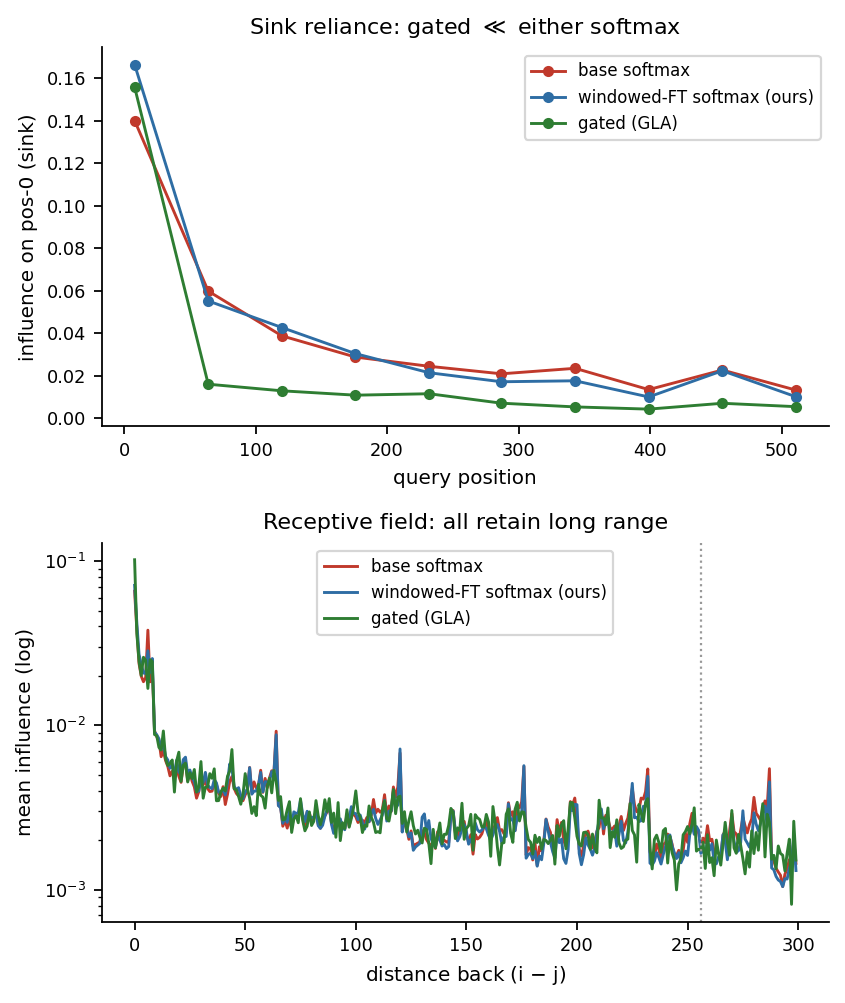
\includegraphics[width=\linewidth]{figures/fla_influence_pattern.png}
\caption{Cross-architecture attention pattern (fla $1.3$B, gradient influence at full attention). \textbf{Left:} the gated model places far less influence on the position-0 sink than either softmax model; base and our windowed-FT softmax coincide --- windowed training does not intrinsically remove the sink, the deployment window does. \textbf{Right:} all three retain long-range influence (overlapping decay); the sink, not the receptive field, is the distinguishing feature.}
\label{fig:infl}
\end{figure}

\subsection{Persistent Prompts as Trainable Sinks}
The persistent-prompt variant ($P{=}64$ always-on prompts $+$ a $W{=}256$ window) lets content tokens spend a controllable fraction of attention on the learned registers: in our run, $19\%$ of every content token's attention goes to the $64$ persistent prompts and $81\%$ to the window. The prompts thus become explicit, trainable attention sinks --- the function the first token was being abused for, now a designed component. On perplexity the persistent and startup variants track the plain windowed model, with a small edge when deployed \emph{narrower} than trained (the prompt fills the coldest part of the window). The registers matter most on a downstream task that needs distant context, which we test with a \emph{fair} control: triangle (full-mask), windowed, and persist models all continued-pretrained on the same wikitext for the same steps, so only the mask differs (Table~\ref{tab:hotpotfair}). At a $256$-token window the full-mask control collapses (HotpotQA generation F1 $0.036$), windowed training recovers it ($0.095$), and the persistent-prompt model reaches $0.166$ --- matching the base$+$StreamingLLM post-hoc trick ($0.166$), but as a trained constant-memory model. This marks the boundary of the broadcasting effect: windowed training spreads attention onto the Type-2 tokens (a distributional change) but does not by itself relay a \emph{specific} distant fact; the persistent registers are what restore long-range anchoring, unifying constant-memory streaming with retrieval in one trained model.

\begin{table}[t]
\centering
\small
\begin{tabular}{llcc}
\toprule
variant (CPT) & deploy & F1 & ans-ppl \\
\midrule
triangle (full-mask) & sliding-history & 0.036 & 112 \\
\textbf{sliding-history} & sliding-history & \textbf{0.095} & 32 \\
\textbf{persist} & persist & \textbf{0.166} & 21 \\
\midrule
base (no CPT) & full & 0.305 & 2.8 \\
base $+$ StreamingLLM & streaming & 0.166 & 13.6 \\
\bottomrule
\end{tabular}
\caption{HotpotQA, \emph{fair} mask-only control (Qwen2.5-0.5B). The three CPT variants see the \emph{same} wikitext for the \emph{same} steps, only the attention mask differs, so QA-ability drift is held constant. At a $256$-token window, the full-mask (triangle) control collapses (F1 $0.036$); sliding-history training recovers it ($0.095$); the persistent-prompt variant reaches $0.166$, \emph{matching the base$+$StreamingLLM post-hoc trick} as a trained constant-memory model. SQuAD-normalised generation F1.}
\label{tab:hotpotfair}
\end{table}


\subsection{Downstream Long-Context QA}
To isolate the mask effect from task learning we also continued-pretrain (no QA supervision) and evaluate zero-shot on LongBench multi-hop QA \citep{bai2024longbench}. At a tight $256$-token window, the windowed model uses its bounded memory markedly better than a full-attention-pretrained control, and StreamingLLM helps the baselines but not the windowed model --- the same signature as in perplexity, on a real task (Fig.~\ref{fig:longbench}).

\begin{figure}[t]
\centering
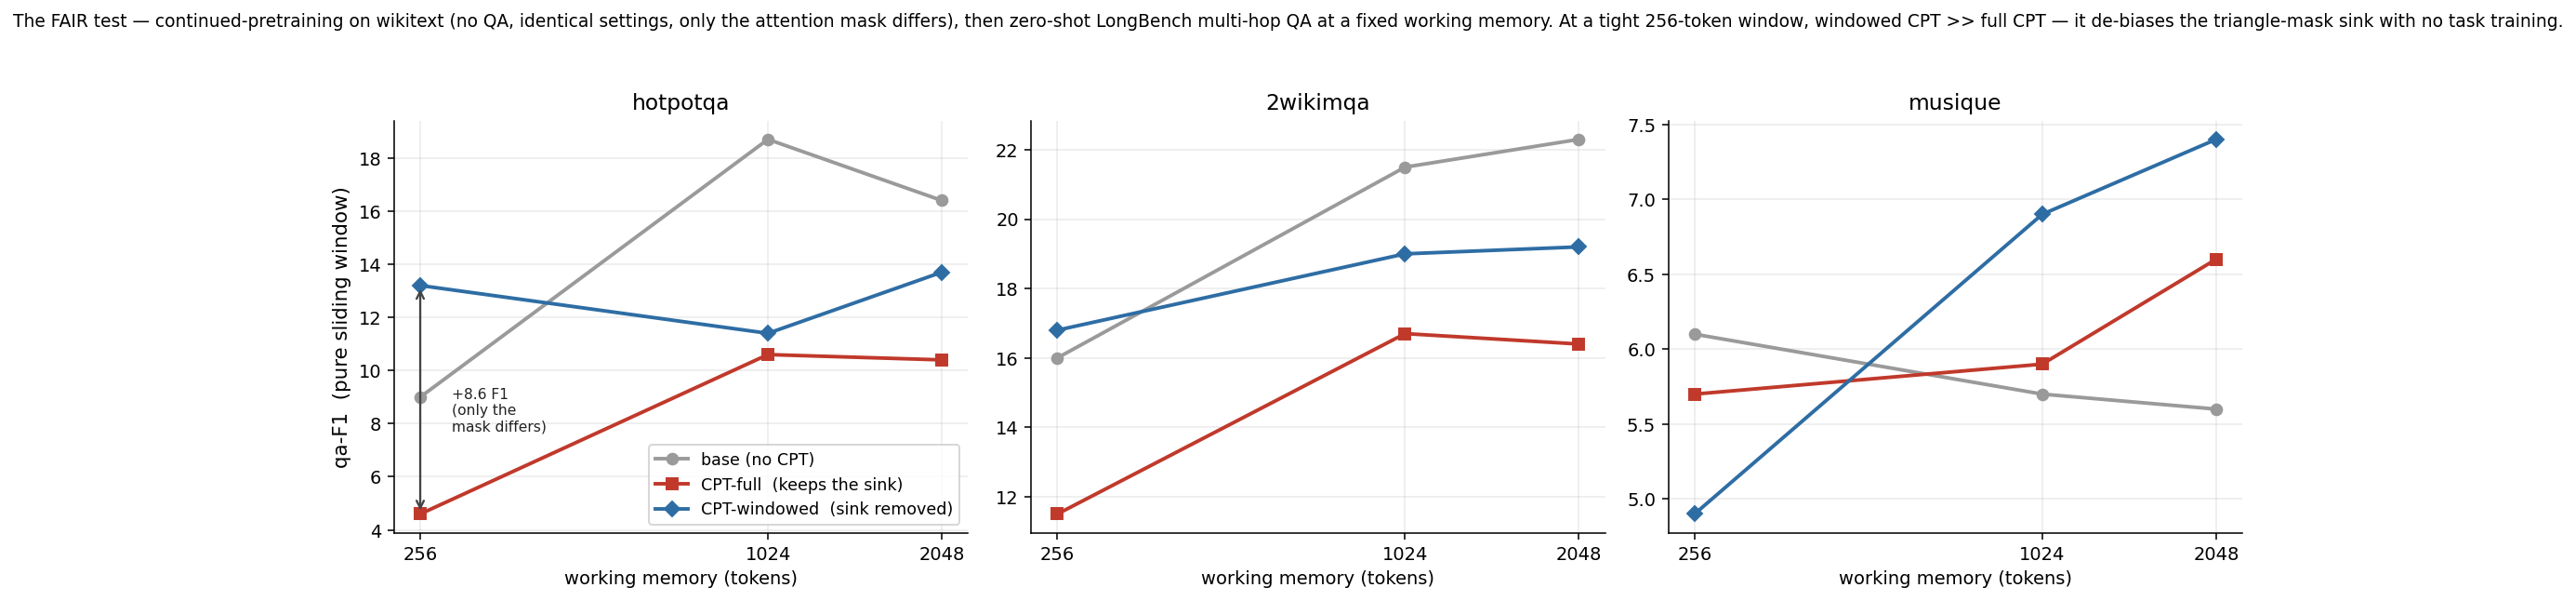
\includegraphics[width=\linewidth]{figures/longbench_cpt_fair.png}
\caption{LongBench multi-hop QA (Qwen2.5-0.5B, continued-pretraining, no task supervision). At a tight window the windowed model uses a bounded working memory better than a full-attention control; the gap shrinks as the window grows.}
\label{fig:longbench}
\end{figure}

\section{Related Work}
\paragraph{Attention sinks and streaming.} \citet{xiao2024streamingllm} identified the sink and exploited it for streaming inference by retaining initial tokens; \citet{han2024lminfinite} use a similar fixed pattern for length generalization. These keep the sink at inference; we remove the dependency by finetuning, and (in the persistent-prompt variant) replace the accidental sink with trainable registers.
\paragraph{Windowed and efficient attention.} Sliding-window attention is used architecturally by Longformer \citep{beltagy2020longformer} and Mistral \citep{jiang2023mistral}, and linear/state-space models \citep{gu2024mamba,gu2025gateddeltanet} achieve constant memory by construction; Qwen3.5 is a hybrid of the two. We instead \emph{finetune} a pretrained softmax model into a windowed one and study what the sink does under that change. Position-extrapolation methods such as ALiBi \citep{press2022alibi} share the ``train short, test long'' spirit; we observe a complementary ``train small, deploy anywhere'' rule for the attention window.
\paragraph{Context as weight.} Our framing --- that windowing forces older context into the parameters --- connects to context distillation and knowledge editing; here the mechanism is attention geometry rather than an explicit distillation loss.

\section{Conclusion}
The attention sink is a learned consequence of the triangular causal mask, and it is exactly what makes a pretrained model fragile to a bounded context. Finetuning under a sliding-window mask removes the dependency: the model acquires a constant working memory, matches full-context quality at a small window, and --- unlike inference-time fixes --- needs no sink tokens. Two design points fall out: ``train small, deploy anywhere,'' and the persistent-prompt variant that turns the accidental sink into a controllable set of trainable registers. We view this as evidence that, for the long-range part of a model's behaviour, context can be traded for weight.

\bibliography{references}

\end{document}
